\section{Beschleuniger-Massensepektrometrie}

Die Beschleuniger-Massenspektrometrie wird von einem Teilchenbeschleuniger unterstützt, indem Teilchen aus einer Probe auf hohe Energien beschleunigt werden.
Ein Vorteil dieser Methode ist es, dass Kernisobare (z. B. $^{10}$Be und $^{10}$B) separiert werden können und dadurch auch geringe Mengen eines Isotops nachgewiesen werden können.
Im Folgenden wird eine detaillierte Beschreibung des Vorgehens anhand des DREAMS am HZDR gegeben.
\begin{figure}[ht]
	\centering
    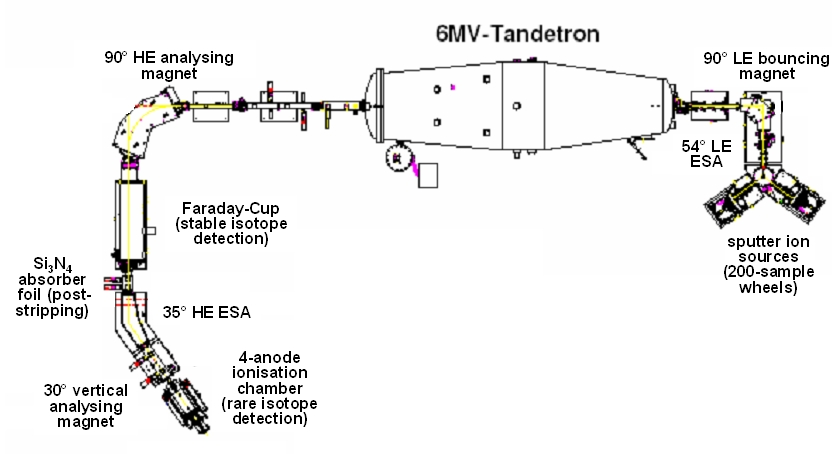
\includegraphics[width=0.95\textwidth]{Pictures/DREAMS.png}
	\caption{Schematik DREAMS \cite{Bild_DREAMS}.}
	\label{Theorie_Bild_DREAMS}
\end{figure}
Die Anlage besteht aus folgenden Komponenten:
\begin{itemize}
    \item Sputter-Ionenquelle
    \item \ang{54} elektrostatischer Analysierer auf der Niederenergieseite
    \item \ang{90} Ablenkmagnet auf der Niederenergieseite
    \item \SI{6}{\mega\volt} Tandem-Beschleuniger
    \item \ang{90} Ablenkmagnet auf der Hochenergieseite
    \item Faraday-Cups zur detektierung stabiler Isotope
    \item SiN Absorberfolie
    \item \ang{35} elektrostatischer Analysierer auf der Hochenergieseite
    \item \ang{30} vertikaler Analysemagnet
    \item Ionisationskammer mit 4 Anoden
\end{itemize}
Wir betrachten als Beispiel die Messung des Isotopenverhältnisses von $^{9}$Be und $^{10}$Be.
Die chemisch aufbereitete Probe befindet sich am Anfang in einer Sputter-Ionenquelle.
Cäsiumatome werden erhitzt, ionisiert und mithilfe einer angelegten Spannung von \SI{7}{\kilo\volt} auf die Probe beschleunigt.
Dabei werden Atome aus dieser gelöst und nehmen Elektronen auf.
Durch eine angelegte Spannung von \SI{29}{\kilo\volt} werden die entstandenen negativen Ionen jetzt beschleunigt.
Mithilfe eines elektrischen Feldes am ESA (elektrostatischer Deflektor) und eines magnetischen Feldes am \ang{90} Magneten werden dabei Ionen unerwünschter Masse (bzw. Ladung) herausgefiltert.
An dieser Stelle wird z. B. das Isotop  $^{9}$Be aus dem Strahl entfernt.
Im Strahl verbleiben das Radioisotop $^{10}$Be und das stabile Isotop $^{10}$Be.
Dieser negative Ionenstrahl, wird danach mit einer Spannung von bis zu \SI{6}{\mega\volt} in die Mitte des Tandem beschleunigt, in welchem sich ein Argon-Gas befindet.
Durch Wechselwirkungen der Ionen mit dem Gas und durch die herrschenden Energien werden verbleibende Moleküle zerstört und Elektronen aus den Ionen geschlagen.
Die jetzt positiven Ionen werden im Tandem weiter zur anderen Seite beschleunigt.
Die Energie der Teilchen nach dem Tandem kann berechnet werden mit:
\begin{gather}
    E_{\text{tot}} = e \cdot (U_{\text{Ionenquelle}} + U_{\text{Beschleuniger}}) \cdot \frac{m_{\text{Ion}^{+}}}{m_{\text{Molekül}^{-}}} + U_{\text{Beschleuniger}} \cdot q_{\text{Ion}^{+}}
    \label{Theo_Energie_nach_Beschleuniger}
\end{gather}
Mit der Elementarladung $e$, der Spannung an der Ionenquelle $U_{\text{Ionenquelle}}$, der Spannung am Tandem $U_{\text{Beschleuniger}}$, der Ionenmasse $m_{\text{Ion}^{+}}$, der Masse der Moleküle $m_{\text{Molekül}^{-}}$ und dem Ladungszustand der Ionen $q_{\text{Ion}^{+}}$.
Im ersten Summand wird der Term $\frac{m_{\text{Ion}^{+}}}{m_{\text{Molekül}^{-}}}$ benutzt um die anteilige kinetische Energie des entstandenen Ions bis zum Argongas zu beschreiben.
Der zweite Summand beschreibt die Beschleunigung nach dem Argongas.
Im Strahlengang nach dem Beschleuniger steht ein weiterer \ang{90} Magnet, durch dessen magnetisches Feld die Isotope nach Impuls (und Ladung) getrennt werden.
Isotope mit hoher Konzentration können jetzt mithilfe eines Faraday-Cup gemessen werden.

Für die Messung der Radioisotope ergibt sich jetzt das Problem, dass einzelne $^{10}$B Isotope im Strahl verbleiben, aufgrund der gleichen Masse und des gleichen Ladungszustands wie das interessante $^{10}$Be Nuklid, was die weitere Messung stören würde.
Um diese Isobare rauszufiltern ist eine dünne Siliciumnitrid-Folie in den Weg des Strahls gelegt.
Der Energieverlust von schweren geladenen Teilchen in dieser Folie berechnet sich mit:
\begin{equation}
E_{loss} = d \cdot \left( \frac{\Delta E}{\Delta x} \right)
\end{equation}
Mit der Dicke der Folie $d$ und dem teilchenspezifischen Energieverlust $\frac{\Delta E}{\Delta x}$.
Der Energieverlust beschreibt mehrere Prozesse gleichzeitig, die zur Abnahme der kinetischen Energie der Ionen führen:
\begin{itemize}
    \item elektronische Abbremsung (inelastische Stöße mit der Elektronenhülle), beschrieben durch die Bethe-Bloch-Formel und für uns meist der dominante Term.
    \item nukleare Abbremsung (elastische Coulomb-Stöße mit den Atomkernen)
    \item Bremsstrahlung
\end{itemize}
Durch den Kernmassen- und Kernladungsabhängigen Energieverlust der Teilchen in der Materie können dann die $^{10}$B Ionen, welche mehr Energie verlieren werden, mithilfe eines elektrischen Feldes in einem weiteren ESA aus dem Strahl entfernt werden.
Gleichzeitig werden innerhalb der Folie weitere Elektronen der Ionen abgezogen, wodurch die Ladung weiter positiv wird (z. B. $^{10}B^{4+}$).
Ein weiterer Magnet lenkt den Strahl dann zu einer Gasionisationskammer (AMS gas-filled ionization chamber in Abb. \ref{Theorie_Bild_DREAMS}), in dem die Ionen mithilfe von vier Anoden (A, B, C, D) in einem Isobutengas ($C_{4}H_{10}$) gezählt werden (siehe Abb. \ref{Theorie_ion_chamber}).
\begin{figure}[ht]
  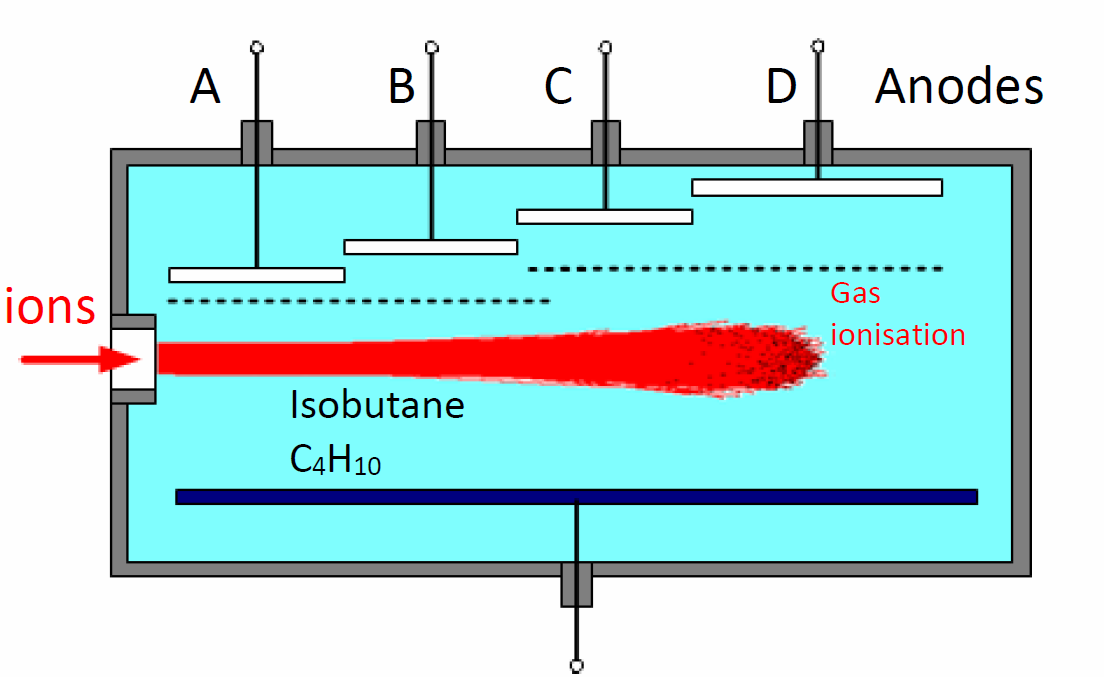
\includegraphics[width=0.95\linewidth]{../Bilder/ion_chamber.png}
  \caption{Gasionisationskammer am DREAMS \cite{Bild_Ionisationskammer}. Die Anoden haben folgende Längen: A - \SI{55.4}{\milli\metre}, B - \SI{49.1}{\milli\metre}, C - \SI{97.6}{\milli\metre}, D - \SI{98.9}{\milli\metre}}
  \label{Theorie_ion_chamber}
\end{figure}
\clearpage
